\documentclass{standalone}
\usepackage{tikz}
\usetikzlibrary{shapes.geometric,shapes.symbols,positioning,decorations.pathmorphing}

%%%%%%%%%%%%%%%%%%%%%%%%%%%%%%%%%%%%%%%%
% you may put a code like this in your .cls file
\tikzset{%
    myblue/.style={blue, very thick},
    pics/bluepoint/.style={code={%          
        \draw[very thick, blue, fill] (0,0) circle [radius=.08];
    }},
    pics/whitepoint/.style={code={%         
        \draw[very thick, blue, fill=white] (0,0) circle [radius = .08];
    }},
    }
\newcommand{\myhelp}{\draw[help lines] (\xmin, \ymin) grid (\xmax, \ymax);}
\newcommand{\mylabels}{%
    \foreach \x in {1} \draw (0,\x)node[right]{\x};
    \foreach \x in {1} \draw (\x,0)node[below]{\x};}
%%%%%%%%%%%%%%%%%%%%%%%%%%%%%%%%%%%%

\begin{document}
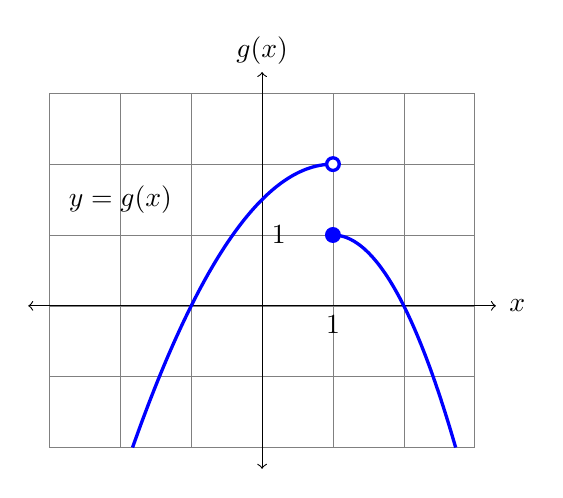
\begin{tikzpicture}[scale=.9]
  \def \xmin {-3}
  \def \xmax {3}
  \def \ymin {-2}
  \def \ymax {3}
  \myhelp  
  \draw [<->] (\xmin-.3,0) -- (\xmax+.3,0);
  \draw [<->] (0,\ymin-.3) -- (0,\ymax+.3);
  \node at (0,\ymax + .6) {$g(x)$};
  \node at (\xmax + .6,0) {$x$};
  \node at (-2, 1.5) {$y = g(x)$};
  \draw[domain=-1.828:1, myblue, smooth] plot
    ({\x}, {-0.5*(\x-1)^2 + 2});
  \draw[domain=1:2.732, myblue, smooth] plot
      ({\x}, {-1*(\x-1)^2 + 1});
  \pic at (1,1) {bluepoint};
  \pic at (1,2) {whitepoint};
  \mylabels
\end{tikzpicture}
\end{document}
